\documentclass{article}

% NeurIPS 2026 style, double-blind workshop track.
\usepackage[dblblindworkshop]{neurips_2026}

\usepackage[utf8]{inputenc}
\usepackage[T1]{fontenc}
\usepackage{hyperref}
\usepackage{url}
\usepackage{booktabs}
\usepackage{amsfonts}
\usepackage{amsmath}
\usepackage{amssymb}
\usepackage{nicefrac}
\usepackage{microtype}
\usepackage{xcolor}
\usepackage{graphicx}
\usepackage{subcaption}
\usepackage{float}
\setlength{\emergencystretch}{2em}
\setlength{\textfloatsep}{11pt plus 2pt minus 4pt}

\title{The Null Problem in SAE Ablations at Vision Transformer Register Tokens}

\workshoptitle{Interpretability as a Science}

\author{%
  Anonymous Author(s) \\
  Affiliation \\
  Address \\
  \texttt{email} \\
}

\begin{document}

\maketitle

\begin{abstract}
Sparse autoencoders are widely used to decompose transformer activations into interpretable features, and a feature's causal importance is commonly established by ablating it and measuring the downstream change. Such a measurement is interpretable only against a null, and we show a token population where no null can both match the ablation's magnitude and stay within the population's own spread. At the register tokens of DINOv2 the five most active features carry a norm of $111.05$ against the register's $110.8$, so the ablation is token deletion; zeroing the position with no autoencoder reproduces its cost to within $0.3\%$. Against energy-matched random controls that deletion is reliably \emph{less} disruptive to downstream patches, on a primary and a held-out cohort and at two model scales, and the ordering reverses at ordinary patch positions. Against the null the population itself supplies, replacing the register with another image's register at the same slot, it is four hundred times \emph{more} disruptive. The two nulls cannot be reconciled here: registers at this slot are near-constant across images, so a perturbation matched to the ablation's magnitude exceeds the population's own spread by a factor of $25$. Which ordering an experiment reports is set by the null it chooses rather than by the features it selects. The geometric statistic offered to explain such effects needs the same scrutiny: a participation ratio pooled over the four register slots reads $1.016$ while the slot an intervention acts on reads $2.98$ and the four-slot mean $15.8$, so the pooled value measures the offset between slots rather than the dimensionality of the population perturbed. We give the within-subpopulation check that separates the two cases, which attention sinks in three language models pass and register slots do not.
\end{abstract}

\section{Introduction}

Sparse autoencoders have become a standard tool for decomposing dense activations into sparse and more interpretable features, and the functional importance of a learned feature is usually argued by ablating it and measuring how far downstream representations move. The features selected for ablation are typically those with the largest activations. This inference leaves a gap, because a large activation establishes that a direction carries magnitude rather than that the model's computation depends on it. Without a control perturbation of comparable size, the reported effect confounds the role of the feature with the effect of perturbing the activation at all. The same gap has been closed elsewhere in interpretability by requiring a matched null, as control tasks do for probing \citep{hewitt2019designing}, and the concern that ablation magnitude and functional importance come apart is itself long-standing \citep{morcos2018importance}. That the choice of null changes what an ablation reports is known \citep{zhang2024towards, miller2024transformer}; we show a population where no choice suffices.

Register tokens in Vision Transformers offer a useful setting in which to examine that gap. \citet{darcet2023vision} introduce them as dedicated non-image tokens that absorb the global computation which would otherwise be carried by high-norm outlier patch tokens, and show that they reduce artifacts, produce smoother feature and attention maps, and improve performance on dense prediction tasks. Because registers carry no fixed spatial correspondence, they provide a token population in which the distinction between a feature being active and a feature being functionally important should be visible.

To examine this, we train a sparse autoencoder in distribution over all $261$ sequence positions of DINOv2-with-registers, so true register positions are seen during training, and ablate its five most active register features against controls matched for perturbation magnitude rather than for selection. Removal is reliably less disruptive than the matched controls, on a primary and an independent held-out cohort and at two model scales, which is the opposite of the ordering the usual reading predicts.

That comparison inverts under a different null. Replacing the register with another image's register at the same slot, the perturbation the population itself supplies, costs $0.018$ points against $7.364$ for removal. Registers there vary so little across images that the two requirements on a null cannot be met together: matching the treatment's magnitude exceeds the population's spread by a factor of $25$, and drawing from that spread gives four percent of the treatment's size. This is the null problem: at such a population the ordering an ablation reports is a property of the null.

The same question applies to the statistic usually offered to explain such effects. The pooled register activation cloud at these layers has a participation ratio of $1.016$, the selected contribution lies almost entirely in its leading direction, and removing it is within $0.4\%$ of removing that direction outright, which invites a geometric reading. That reading needs the statistic to describe the population an intervention acts on, and the pooled value does not. It averages four register slots whose means differ, and the separation between slots is what drives it toward one; the slot the ablation acts on reads $2.98$, and the four-slot mean $15.8$. Across $22$ layers of two models the association between dimensionality and the ablation effect changes sign with the definition used, so no dimensionality-based prediction of the effect follows from the pooled quantity.

The two results share a structure: a quantity that appears to characterise the intervention, the size of a perturbation and the dimensionality of the cloud it acts in, is instead fixed by a property of the population it is measured against. Applying the same measurement to attention-sink tokens in three language models shows the second case is specific rather than general, since a sink is a single position and nothing is pooled, and there the dimensionality gap survives both a sample-size-matched and a position-demeaned control. The distinction is what a practitioner needs in order to know when the diagnostic can be trusted.

Our contributions are threefold. First, we show that a standard top-$k$ ablation at register positions is token deletion, that its ordering against a null is set by the choice of null, and that neither null we construct matches both magnitude and support, the population's own spread bounding how well any can; the intervention result replicates across cohorts and model scale, and the selection rule is input-invariant because one register slot carries fourteen times the norm of the others. Second, we rule out the accounts that follow from registers being attention sinks, no scalar measure of perturbation size ordering the effects. Third, we show that a participation ratio pooled over subpopulations with different means reports their separation rather than their dimensionality, and give the within-subpopulation check that separates the cases where it can be trusted from those where it cannot.

\section{Related Work}

\textbf{Outlier Tokens and Register Tokens.} Self-supervised Vision Transformers based on DINO \citep{caron2021emerging} and DINOv2 \citep{oquab2023dinov2} learn rich structure without explicit supervision, but at scale their attention and feature maps develop localized high-norm artifacts on around $2\%$ of patch tokens, hypothesized to accumulate global information rather than local content; \citet{darcet2023vision} introduced register tokens as dedicated non-image positions providing capacity for that computation. More recent work argues these artifacts follow from the softmax bottleneck, in which a few tokens carry disproportionate residual attention mass \citep{jiang2025vision}; that work also reproduces the register benefit with no trained register apparatus.

\textbf{Sparse Autoencoders.} SAEs decompose dense activations into a sparse set of more interpretable latents \citep{cunningham2023sparse}; much of the literature is on text \citep{gao2024scaling, templeton2024scaling}, and vision use is growing \citep{fel2025archetypal}. A parallel line asks what SAE-based evidence establishes, developing principled evaluations that hold the intervention fixed \citep{makelov2024principled} and showing that SAE pipelines return apparently interpretable structure even on randomly initialized transformers \citep{heap2025sparse}. Our contribution is to that line.

\textbf{What an ablation is measured against.} The circuit literature establishes that a result depends on the distribution patched in: causal scrubbing resamples from a reference distribution rather than zeroing \citep{chan2022causal}, and varying the corruption alone changes which components a study localizes and how faithful a circuit appears \citep{zhang2024towards, miller2024transformer, heimersheim2024how}. That work treats the null as a choice to be made well. Concurrent work finds in language models that SAE ablations look localized or not depending on the matched baseline \citep{luo2026when}; we isolate a vision population where the matching itself is obstructed rather than merely consequential.

\textbf{Representation geometry.} That transformer activation spaces are strongly anisotropic is well established: contextual embeddings occupy narrow cones \citep{ethayarajh2019contextual, gao2019representation}, a few rogue dimensions dominate similarity structure until removed \citep{timkey2021bark}, and stripping dominant directions is standard postprocessing \citep{mu2018allbut}. What that literature shows about the validity of similarity measurements, we show about the validity of ablation measurements.

\textbf{Special tokens and massive activations.} Outside vision, \citet{xiao2023efficient} show that the first positions of a language model absorb disproportionate attention mass and \citet{sun2024massive} document outsized-norm activations on a few tokens and dimensions. These populations are frequent subjects of interpretability claims, which is why Section~\ref{sec:generality} measures their geometry directly rather than reasoning by analogy.

\section{Method}
\label{sec:method}

\subsection{Two token populations}
\label{sec:populations}

\textit{facebook/dinov2-with-registers-small} inserts four register tokens immediately after the CLS token, so at the layer-8 hook used throughout (the output of Hugging Face encoder block index 8, zero-based) the $261$ sequence positions are CLS at $[0{:}1)$, four registers at $[1{:}5)$, and $256$ patch tokens at $[5{:}261)$. We verified this at the hook rather than assuming it from variable names.

Our design applies the same intervention protocol to two token populations drawn from the same model, the same layer, and the same images, which differ sharply in the geometry of their activation clouds: at layer 8 the register cloud has an effective dimensionality of $15.8$ against $123.6$ for the patch cloud at the same layer, each measured within position. Computed the way such statistics usually are, by pooling the four register slots, the register figure instead reads $1.016$; Section~\ref{sec:artifact} takes up why the two differ by an order of magnitude. The contrast that motivates the design holds under either. The first consists of the true registers at $[1{:}5)$. The second consists of the four terminal patch positions $[257{:}261)$, which are ordinary patch tokens carrying image-local content. For the terminal-patch population we use a separate SAE trained on exactly those four positions, which fits them at an explained variance of $0.661$ and is what makes it usable here as a well-fit model of an ordinary, non-register population. Appendix~\ref{app:provenance} records how its training population was established.

\subsection{Sparse autoencoders}
Before SAE training, we normalize activations by a global scalar $\sigma = \sqrt{\mathbb{E}[\|x\|_2^2]}$ computed over the training activations for each token subset, so that normalized activations have unit expected squared norm.

Each SAE encodes the normalized activation into a sparse latent representation using a TopK nonlinearity that retains only its $k$ largest pre-activations,\footnote{Verified against the stored checkpoint configurations (\texttt{AutoEncoderTopK}, \texttt{dict\_size: 2048}, \texttt{k: 6} throughout) rather than the training script's comments, which describe a ReLU encoder with a separate $\ell_1$ penalty and do not match the trained artifact.}
\[f(x) = \operatorname{TopK}_{k}\!\left(\operatorname{ReLU}\left(W_{\mathrm{enc}}(x - b_{\mathrm{dec}}) + b_{\mathrm{enc}}\right)\right),\]
and reconstructs the activation through the decoder:
\[\hat{x} = W_{\mathrm{dec}} f(x) + b_{\mathrm{dec}} .\]
Every SAE in this study uses a dictionary of $2{,}048$ decoder directions with $k=6$, and is optimized to minimize mean-squared reconstruction error; the TopK nonlinearity enforces sparsity directly, so no separate sparsity penalty is added to the loss. We report fit quality as the fraction of variance explained, $\mathrm{FVE} = 1 - \operatorname{Var}(x - \hat{x}) / \operatorname{Var}(x)$. Removing the top five of six active latents is a large fraction of the code; Section~\ref{sec:limitations} states what that implies for SAEs operating at larger $k$.

\subsection{Intervention and endpoint}
\label{sec:intervention}

For each image we compute the SAE latent representation $f(x)$ at the intervened positions, identify the five features with the largest positive activations, and subtract their decoder contribution. At registers that contribution is nearly the whole token, at norm $111.05$ against the register's $110.8$ and cosine $0.9998$ with it, so the intervention is token deletion. Zeroing the register with no autoencoder costs $7.342$ points, a paired difference of $0.021$ from top-five removal's $7.364$ (CI $[+0.002,+0.038]$), so the dictionary determines $0.3\%$ of the effect. We then re-execute the blocks after the hooked layer and the final layer norm exactly. The endpoint is the mean percentage-point drop in cosine similarity between clean and intervened final-layer patch representations, with $10{,}000$-resample paired bootstrap $95\%$ confidence intervals over images. The patch metric excludes the intervened positions themselves.

\subsection{A graded family of matched controls}
\label{sec:controls}

Because a large activation does not by itself establish that a feature matters more than an arbitrary perturbation of the same size, we compare selected-feature removal against controls matched for perturbation magnitude rather than for selection. Every control below is rescaled to carry exactly the energy of the selected contribution, so the conditions differ only in \emph{where} the perturbation points, never in how large it is.

Let $V_r$ hold the top $r$ principal directions of the intervened population's activation cloud, estimated over the cohort. The controls form a ladder indexed by how much of the ambient space the perturbation is drawn from. \emph{Aligned $V_1$} is the selected contribution's own projection onto $V_1$, rescaled to the selected energy, which is the largest leading-PC removal of that size; comparing it against selected-feature removal isolates the SAE's contribution from the geometry's. \emph{Random within $V_4$} is a random direction inside the top four principal directions. \emph{Random decoder span} is a random direction built from the decoder dictionary, and \emph{decoder permutation} keeps the selected support and coefficients while replacing only the decoder columns; neither is aligned with the population's leading directions. We also report a \emph{sign-flipped} condition that adds the identical vector instead of subtracting it, and a \emph{random within $V_1$} condition. Randomized controls are averaged over eight draws per image before bootstrapping. The ladder varies direction at fixed magnitude. We also run the null the population itself supplies, replacing the intervened register with another image's register at the same slot, unscaled, which matches support exactly and magnitude not at all.

\subsection{Experimental setup}
\label{sec:setup}

All SAEs are trained on layer-8 residual-stream activations from ImageNet-1k, with activation dimension $384$ at Small and $768$ at Base. The primary cohort is a fixed $512$-image ImageNet validation sample, and the holdout an independent $256$-image sample drawn later in the same stream. Controls use eight draws per image. Cross-scale replication uses DINOv2-Base, with a full-token SAE trained under a matched compute budget. Participation ratios are computed as $(\sum_i \lambda_i)^2 / \sum_i \lambda_i^2$ over the eigenvalues of the centered covariance of the relevant activation cloud, a standard summary of effective dimensionality that equals $1$ for a rank-one cloud and $d$ for an isotropic one.

\section{Selected-Feature Removal Under Matched Controls}
\label{sec:main}

The full-token SAE reconstructs true registers at an explained variance of $0.999$, so reconstruction is not a meaningful confound here, and injecting its reconstruction with no feature removed costs $0.224$ points (CI $[0.211,0.237]$). Against that baseline clean top-five removal costs $7.364$ points, yet is $6.792$ points \emph{less} disruptive than the energy-matched random decoder-span control and $5.364$ points less than the decoder-permutation control.

\begin{table}[t]
\centering
\caption{Matched-control contrasts at true registers and at terminal patches, both model scales and both cohorts. Values are the mean percentage-point difference between clean top-five removal and the matched control, so a negative value indicates that removal is \emph{less} disruptive. All sixteen intervals exclude zero; they are given in full in Appendix~\ref{app:numbers}.}
\label{tab:replication-grid}
\begin{tabular}{llrrrr}
\toprule
& & \multicolumn{2}{c}{vs.\ random span} & \multicolumn{2}{c}{vs.\ permutation} \\
\cmidrule(lr){3-4}\cmidrule(lr){5-6}
Scale & Positions & primary & holdout & primary & holdout \\
\midrule
Small & registers $[1{:}5)$    & $-6.792$  & $-6.670$  & $-5.364$  & $-5.016$ \\
Base  & registers $[1{:}5)$    & $-4.807$  & $-4.680$  & $-7.444$  & $-6.960$ \\
Small & terminal $[257{:}261)$ & $+0.0074$ & $+0.0073$ & $+0.0084$ & $+0.0071$ \\
Base  & terminal $[257{:}261)$ & $+0.0055$ & $+0.0065$ & $+0.0072$ & $+0.0076$ \\
\bottomrule
\end{tabular}
\end{table}

\textbf{The selected support is input-invariant, and one slot is why.} At true registers the same five dictionary coordinates, all on a single register slot, are selected for every image in both cohorts and at Base scale. Mean register norms at the four slots are $7.5$, $110.8$, $7.9$ and $7.4$, so the top five over the flattened grid must fall on the second slot for every image; the invariance follows from that offset rather than from the dictionary. At terminal patches the identical rule is almost perfectly image-specific, returning $510$ distinct sets across $512$ images from $566$ distinct latents spread over all four positions. Coefficients on those coordinates do vary with the image, so the ablation vector is not identical across inputs: its norm ranges $99.3$ to $117.3$ about a mean of $111.1$. What is input-invariant is the \emph{choice} of what to ablate, which is the part a feature-importance reading depends on.

\textbf{The ordering reverses at ordinary patch positions, and replicates at a second scale.} Table~\ref{tab:replication-grid} gives the full grid. At terminal patches the identical rule and controls give the ordinary expected ordering on both cohorts at both scales; at registers the sign is negative in all four rows. The register effects are three orders of magnitude larger, and the two SAEs differ in fit ($0.999$ against $0.661$), so that arm establishes a sign and not a magnitude: fit bounds how much of a token an ablation removes, not which side of a matched control it falls on.

\section{The Geometry of the Intervention and Its Nulls}
\label{sec:geometry}

At layer 8 a participation ratio pooled over the four register slots reads $1.016$ against $120.6$ for the patch cloud at the same layer, and Section~\ref{sec:artifact} takes up what that pooled number measures. The selected contribution lies almost entirely inside its leading direction, carrying $99.7\%$ of its squared norm there, while the energy-matched random span lies almost entirely outside it at $0.6\%$ (paired difference $0.991$, CI $[0.991,0.992]$).

\textbf{The cloud is two clusters.} Resolved along its leading direction, three of the four registers sit together at a coordinate of $+27.4$ and the fourth at $-82.1$, so the participation ratio of $1.016$ reflects that separation rather than a one-dimensional continuum. The five selected latents lie on the outlying register for every image, and removing their contribution moves it from $-82.1$ to $+28.8$, crossing the population mean and landing where the other three sit.

\begin{table}[t]
\centering
\caption{The control ladder at true registers, DINOv2-Small, layer 8. Ladder interventions carry the same perturbation energy and differ only in direction. \emph{Post-LN} is $\|\mathrm{LN}(r')-\mathrm{LN}(r)\|$, the displacement the next block receives; none of the last three columns orders the costs. Contrast is clean top-five removal minus the control. The final block leaves the ladder: zeroing uses no autoencoder and the swap conditions match support rather than energy; it is a separate run whose own clean cost is $7.364$, with contrasts paired within run, and unlike the ladder it was measured only at Small, layer 8, primary cohort. Primary cohort, $n=511$ (norm and attention, $n=128$); all intervals exclude zero and every ladder cost replicates on the holdout.}
\label{tab:ladder}
\footnotesize
\setlength{\tabcolsep}{3.5pt}
\begin{tabular}{lrrrrrr}
\toprule
Condition & Cost & Contrast & 95\% CI & Post-LN & Norm & Attn. \\
\midrule
No intervention                 & ---      & ---      & ---                & ---      & $110.8$ & $0.185$ \\
Sign flip (add, not subtract)   & $0.227$  & $+7.137$ & $[+6.978, +7.297]$ & $0.44$   & $221.8$ & $0.198$ \\
Random within $V_1$             & $3.714$  & $+3.650$ & $[+3.509, +3.796]$ & $16.70$  & ---     & ---     \\
\textbf{Clean top-five removal} & $7.363$  & ---      & ---                & $32.99$  & $4.2$   & $0.000$ \\
Aligned $V_1$ (leading-PC)      & $7.393$  & $-0.030$ & $[-0.042, -0.017]$ & $39.19$  & ---     & ---     \\
Random within $V_4$             & $8.867$  & $-1.504$ & $[-1.690, -1.322]$ & $19.26$  & ---     & ---     \\
Decoder permutation             & $12.727$ & $-5.364$ & $[-5.588, -5.143]$ & $19.32$  & ---     & ---     \\
Random decoder span             & $14.155$ & $-6.792$ & $[-7.048, -6.538]$ & $19.20$  & $156.5$ & $0.104$ \\
\midrule
Zero the register (no SAE)       & $7.342$  & $+0.021$ & $[+0.002, +0.038]$ & ---      & ---     & ---     \\
Swap with another image (on support) & $0.018$ & $+7.346$ & $[+7.185, +7.511]$ & ---   & ---     & ---     \\
Same swap, rescaled to treatment energy & $10.519$ & $-3.156$ & $[-3.722, -2.617]$ & --- & ---   & ---     \\
\bottomrule
\end{tabular}
\end{table}

\textbf{Cost rises with the dimensionality of the subspace the perturbation is drawn from.} Holding perturbation energy exactly fixed, cost rises monotonically with the dimensionality of the subspace the perturbation is drawn from, at $7.393$, $8.867$ and $14.155$ points for the leading direction, the top four, and the full $384$-dimensional stream (Table~\ref{tab:ladder}); the ordering replicates on the holdout. This ordering is what a geometric account predicts and a feature-specific one does not. The conditions differ in alignment and construction as well as in dimensionality, so we report the ordering rather than attribute it to dimensionality alone.

\textbf{The sparse autoencoder contributes little at this operating point.} Removing the leading principal component, rescaled to the selected energy, costs $7.393$ points against $7.363$ for removing the five selected features; the difference is reliable but small, at roughly $0.4\%$ of the effect, and the near-equivalence replicates on the holdout. That is close to what a rank-one cloud entails, and the content is that top-$k$ selection recovers the pooled cloud's dominant direction rather than feature-specific structure.

\textbf{None of four scalar measures of perturbation size orders the conditions.} Our controls equalize magnitude in the residual stream, but DINOv2 applies LayerNorm before attention, so the next block sees $\mathrm{LN}(r')$ and equal residual-stream magnitude is not equal magnitude there. Measuring $\|\mathrm{LN}(r')-\mathrm{LN}(r)\|$, the conditions of Table~\ref{tab:ladder} span $0.44$ to $39.19$ despite identical residual-stream energy. That does not rescue a magnitude account: the three costliest receive near-identical displacements of $19.26$, $19.32$ and $19.20$ while their costs span a factor of $1.6$, and removal displaces the interface $1.7$ times more than the random span while costing half as much. Two further scalar accounts fail alike. Addition changes the register's norm most, at $+100\%$, and is cheapest; the random span changes it least, at $+41\%$, and is dearest. The register is genuinely a sink, taking $18.5\%$ of patch attention, yet removal destroys that mass entirely at $7.364$ while the random span removes $44\%$ of it at nearly twice the cost. None of these four ways of asking whether two perturbations are the same size orders these effects.

\textbf{Magnitude matching and support matching cannot both be had here.} Every control above is matched on magnitude but drawn from a direction the model never encounters there: a random decoder direction of norm $111$ applied to a token of norm $111$ is close to replacing the token with noise, so its greater disruption may register only sensitivity to leaving the distribution. The null that reasoning calls for is drawn from the empirical distribution at the same slot. Replacing the intervened register wholesale with another image's register at that slot is exactly that, and it costs $0.018$ points against $7.364$ for selected-feature removal (paired difference $+7.346$, CI $[+7.185,+7.511]$, eight draws per image). Against an on-support null the ordering is not reversed but inverted, removal being some four hundred times more disruptive than the largest perturbation the population actually supplies.

The two nulls cannot be reconciled, and that is the result. Registers at this slot are near-constant across images, so the difference between two of them has a norm of $4.60$ against the treatment's $111.05$. Rescaling that difference to the treatment's energy, the other way to build a null from the population's own directions, amplifies it $25.4$ times on average (range $7.7$ to $38.0$) and costs $10.519$ points, above the treatment again. A perturbation of the treatment's magnitude is necessarily off support here, and one on support is four percent of that magnitude and nearly free. Where a population is this degenerate the two requirements pull apart, so the ordering an ablation reports turns on which of them its null was built to satisfy.


\section{What the Pooled Participation Ratio Measures}
\label{sec:artifact}
\label{sec:crosslayer}

Effective dimensionality is the statistic usually offered to explain effects of this kind, and at a special-token population it is usually computed by pooling the positions that make it up. That pooling is not innocuous.

\textbf{The pooled statistic measures the offset between slots.} A participation ratio over all four register positions pools subpopulations whose means differ, and a difference in means inflates the leading eigenvalue whether or not any subpopulation is degenerate. At layer 8 of DINOv2-Small the pooled ratio is $1.016$, while within each slot across images it is $20.2$, $3.0$, $20.9$ and $19.0$, and after subtracting each slot's own mean it is $18.7$ (Table~\ref{tab:slots}, Figure~\ref{fig:artifact}a). The two protocols touch different slots: the top-five removal of Section~\ref{sec:main} acts on one slot, whose own ratio is $2.98$, and the sweep below on all four, for which the matching value is the $15.8$ slot-wise mean. A ratio of $2.98$ in $384$ dimensions is still very low-dimensional, and it is the lowest of the four slots at both scales, Base selecting slot $3$ at $7.92$ against a four-slot mean of $17.8$, so a geometric account stated over the \emph{intervened slot} remains available. What the pooled value cannot do is supply the evidence for it: $1.016$ is not a measurement of that slot, and the near-degeneracy it reports is largely the offset between slots.

The two-cluster structure of Section~\ref{sec:geometry} is the same fact from the other side: the leading pooled direction is essentially the indicator of which slot a vector came from, and the location removal moves the register to is one the model meets \emph{at slots 0, 2 and 3}, never at the intervened slot.

\begin{figure}[t]
\centering
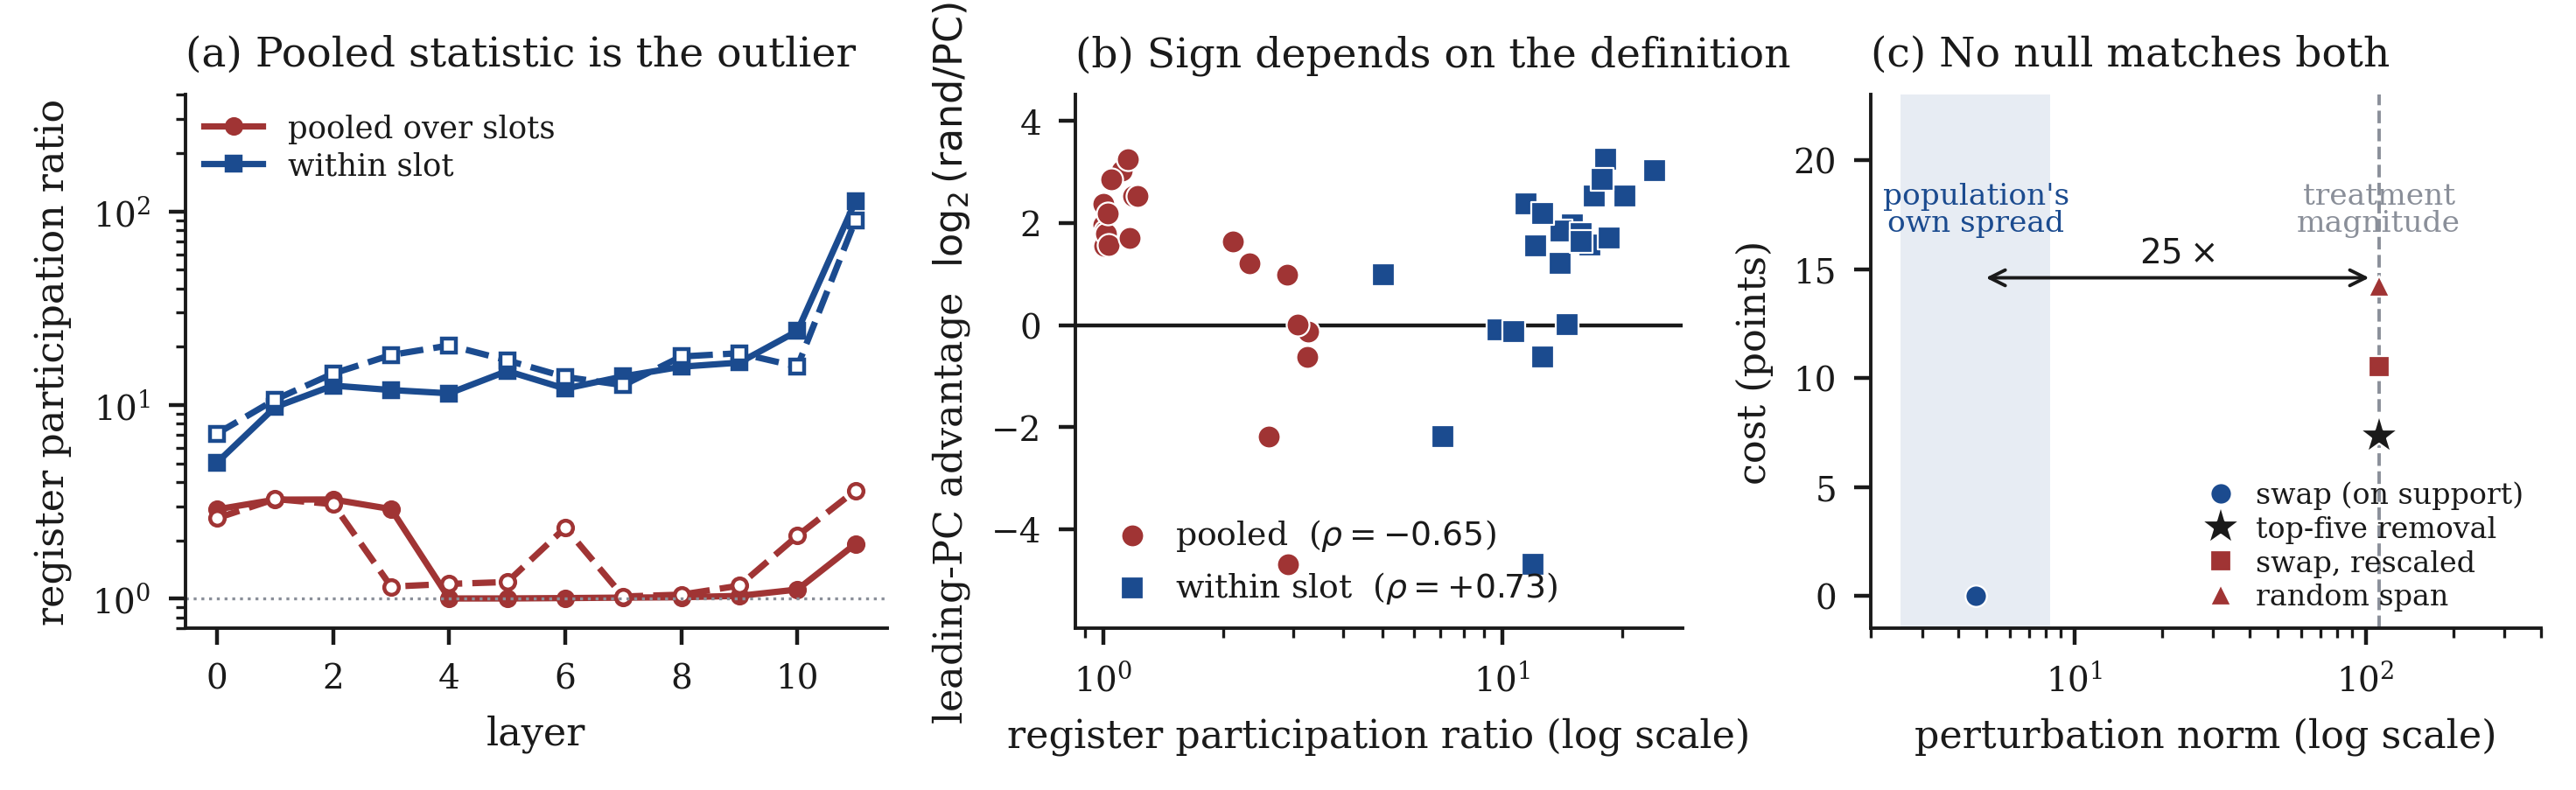
\includegraphics[width=0.94\textwidth]{figure_pooling_artifact.png}
\caption{(a) The register participation ratio across depth, pooled over the four slots and computed within slots. The pooled statistic sits near one through the middle layers while the within-slot value is an order of magnitude larger, so it tracks the offset between slots rather than the dimensionality of the population an intervention acts on. (b) The consequence, over the $22$ non-vacuous layers of both models. The leading-PC advantage falls with the pooled ratio and rises with the within-slot ratio, so the sign is set by which definition is used. (c) The matching problem at layer 8 of Small: the perturbation the population supplies has norm $4.60$ and is nearly free, while every control matched to the treatment's $111.05$ sits a factor of $25$ outside that spread. Small is solid and filled, Base dashed and open.}
\label{fig:artifact}
\end{figure}

\textbf{The cross-layer relationship reverses with the definition.} We ran the geometric intervention SAE-free at every layer of both models, stripping each register's component along the leading direction of its own cloud against an energy-matched random control, and summarize it as $A_\ell = \log_2(\text{rand}_\ell/\text{PC}_\ell)$ so layers whose absolute effects differ by two orders of magnitude stay comparable. Against the pooled participation ratio $A_\ell$ falls at Spearman $\rho = -0.65$ over $22$ layers, the relationship the geometric account predicts. Against the mean within-slot ratio of the same layers it rises, at $\rho = +0.73$; against the slot-demeaned ratio it rises more weakly, at $\rho = +0.41$. The interventions and endpoints are identical across all three; only the predictor's definition changes. The reversed correlations do not by themselves carry a per-slot account: the sweep removes the \emph{pooled} leading component from all four slots rather than the per-slot component such an account calls for, and the correlations run over $22$ layers that are two models by eleven depths, independent along neither axis. The claim is the narrow one. The pooled participation ratio is not a measurement of the population any single intervention acts on, so it cannot support a dimensionality-based prediction; whether a per-slot version can is open, and the experiment that would settle it, fitting per-slot geometry on one cohort and intervening slot-wise on the other, we have not run.

The intervention results of Sections~\ref{sec:main} and \ref{sec:geometry} are measured contrasts between conditions and do not depend on this statistic. What remains open is the explanation, and the reason belongs to the diagnostic rather than to the intervention.

\section{The Same Measurement Where It Is Not Confounded}
\label{sec:generality}

Section~\ref{sec:artifact} shows the statistic reporting a between-slot offset; here it reports what it is meant to, which makes the two cases diagnosable. A sink is a \emph{single} position, so nothing is pooled. We apply the identical measurement, with the sink in the role of the register and positions from index 8 onward in the role of the patches, over $512$ wikitext-103 paragraphs truncated to a $128$-token context (Appendix~\ref{app:repro}); no SAE or intervention is involved.

\begin{table}[t]
\centering
\caption{Effective dimensionality of special-token and ordinary-token activation clouds. Vision rows are measured at layer 8, language rows at the layer indicated. The norm ratio is the mid-layer mean $L_2$ norm of the special over the ordinary population. Vision rows report the \emph{intervened} slot, the one position the top-five rule selects for every image and the analogue of a sink; four-slot means are $15.8$ and $17.8$, pooled values $1.02$ and $1.05$. The patch column is position-demeaned for symmetry with the language rows, moving it from $120.6$ to $123.6$. Language rows need no correction on the special-token side, a sink being a single position.}
\label{tab:generality}
\begin{tabular}{lrrrr}
\toprule
Model & Special PR & Ordinary PR & Gap & Norm ratio \\
\midrule
DINOv2-Small (L8)   & 2.98 & 123.6 & $41\times$  & --- \\
DINOv2-Base (L8)    & 7.92 & 190.9 & $24\times$ & --- \\
Qwen2.5-0.5B (L8)   & 1.15 & 113.7 & $99\times$  & $98.6\times$ \\
GPT-2 (L8)          & 2.50 & 147.5 & $59\times$  & $34.6\times$ \\
Pythia-160m (L7)    & 2.00 & 4.0   & $2\times$   & $15.3\times$ \\
\bottomrule
\end{tabular}
\end{table}

Near-one-dimensional special-token geometry is not particular to vision. The sink in Qwen2.5-0.5B holds a participation ratio below $1.20$ across nineteen consecutive layers, with the collapse and re-expansion with depth that DINOv2 registers show (Appendix~\ref{app:llm}); GPT-2's is $59$ times lower-dimensional than its ordinary tokens without being close to one-dimensional, at $2.50$.

These gaps are not a sample-size artifact. A sink contributes one vector per sequence, so its cloud holds under $500$ vectors in $768$ to $896$ dimensions against around $59{,}000$ for ordinary tokens, and the participation ratio is biased downward at small $n$, in the direction that favours our conclusion. Re-estimating the ordinary ratio from one token per sequence, at the sink's own sample size, leaves both gaps intact: Qwen falls from $99\times$ to $80\times$ and GPT-2 from $59\times$ to $45\times$ over $20$ draws. Nor is the ordinary side inflated by pooling, the failure mode of Section~\ref{sec:artifact}: subtracting each position's own mean moves the ratio from $113.7$ to $113.4$ in Qwen, $147.5$ to $150.2$ in GPT-2 and $3.99$ to $3.98$ in Pythia. Where the populations compared are single positions, or pooled over positions whose means barely differ, the statistic behaves.

Pythia-160m is the case the control does not clear. Its full-sample ordinary estimate ($n=58{,}080$) puts the whole residual stream near a participation ratio of $4$. What the matched-$n$ exercise shows is how poorly the statistic is determined \emph{at the sample size a sink supplies}: drawn at $n\approx480$ that same population yields anything from $2.1$ to $35.7$ across $20$ draws. Since a sink is only ever measured at that size, it is the sink's estimate here that cannot be trusted, not the ordinary one. The instability is diagnostic: in a separate variance audit ($n=29{,}640$) the largest-variance dimension carries $38.7\%$ of the total and the max-to-median per-dimension variance ratio is $721$, the rogue dimensions of \citet{timkey2021bark}, which a draw either catches or does not. We therefore do not report Pythia as a negative case but as a second condition on the check: where a few rogue coordinates dominate, the participation ratio is not identified at the sample sizes a special-token population supplies.

\textbf{Norm is a poor proxy for dimensionality.} The sink in Pythia carries $15.3$ times the norm of its ordinary tokens with only a twofold gap in dimensionality, while the sink in Qwen carries $98.6$ times the norm with a $99$-fold gap. The two are rank-concordant across our three models, so we do not claim they dissociate; they are far from proportional, a sixfold spread in norm ratio spanning a fiftyfold spread in dimensionality gap, so norm does not calibrate dimensionality even where it predicts its direction. This bears on identifying special tokens by norm, including the high-norm outlier criterion: it does not establish whether an ablation there is evidence about features.

\section{Discussion}

Two consequences follow. A null must match the treatment's magnitude to bound the effect of perturbing at all, and must lie in the population's support to bound the effect of leaving the distribution. Where a token population is near-constant those requirements pull apart, and an ablation returns whichever ordering its null was built to return. The test is cheap and needs no harness: compare the treatment's norm against the spread of the population it acts on, where a ratio of $25$ says in advance that no null will satisfy both.

The second belongs to the diagnostic rather than to the intervention. Effective dimensionality over a special-token population is interpretable only if the population is homogeneous in the mean, and register slots are not, so pooling them manufactures a leading direction that is the slot indicator. The check is the same eigendecomposition computed within subpopulations: sinks pass trivially, being one position; register slots do not.

The natural alternative, that cost is set by norm or attention mass rather than direction, is tested in Section~\ref{sec:geometry}, and neither orders the effects. What remains unseparated is finer: attention mass at one block does not capture how the perturbed key interacts with individual query heads.

None of this is evidence that register directions are unimportant: moving a register to a location other registers occupy is not the same as removing information the model uses.

\section{Limitations}
\label{sec:limitations}

Our endpoint is representational, the cosine similarity between clean and intervened final-layer patch representations, so we can say removal changes downstream representations less than matched controls do without establishing what that implies for a task. A probe-based endpoint is the natural next step.

Our SAEs use $k=6$, so removing five features removes most of the active code; this speaks to small-$k$ operating points, and whether the reversal survives ablating one feature of sixty-four is not established. Registers are four of $261$ training positions, so whether an SAE trained on $[1{:}5)$ alone reproduces the behaviour is the single most informative experiment we have not run. We train one SAE per configuration and vary neither seed nor dictionary size. Our two nulls bracket rather than resolve the matching problem: we show the requirements pull apart for the constructions we tested, not that none can satisfy both, and conditional or covariance-aware resampling we do not attempt. The swap and zeroing comparisons were run only at Small, layer 8, primary cohort. Our register participation ratios use one vector per image per slot while the patch ratios draw on many positions per image, an asymmetry the language-model section controls for and the vision section does not.

Our causal interventions are confined to vision, so the claim that crosses architectures is a claim about measurement rather than about mechanism. We make no prediction about ablation effects in language models, since no account established here licenses one.

We report no validated explanation of the effects measured here. Section~\ref{sec:artifact} shows the pooled statistic cannot supply a dimensionality-based account, and the within-slot relationship runs in the opposite direction.

\section{Conclusion}

Removing the five most active register features of DINOv2 removes the register, and is less disruptive than an equal-norm random vector on two cohorts and two scales, reversing at ordinary patches. Against the perturbation the population itself supplies it is four hundred times more disruptive. Both comparisons are sound and they disagree, because at a token that barely varies across inputs the two requirements on a null pull apart. The statistic offered to explain such effects has the same shape: a participation ratio pooled over four slots with different means measures their separation, not the dimensionality of the population an intervention acts on. In each case the quantity that looks like a property of the intervention is fixed by the population it is measured against, and one cheap comparison says in advance which reading the measurement will support.

\bibliographystyle{plainnat}
\bibliography{references}

\section*{NeurIPS Paper Checklist}
\begin{enumerate}
\item \textbf{Claims.} \answerYes{} The abstract and introduction state the matched-control finding (selected register-feature removal is reliably less disruptive than energy-matched controls and reliably more disruptive than an on-support null), that no null at this population matches both magnitude and support, that the rule selecting what to ablate is input-invariant while its coefficients are not, that norm and attention-mass accounts are ruled out, and that the geometric account is not supported by the pooled statistic offered for it. We explicitly report no dimensionality-based prediction of the effect. Claims are restricted to the tested models, SAEs, layers, cohorts, and metric.
\item \textbf{Limitations.} \answerYes{} Section~\ref{sec:limitations} states that the endpoint is representational rather than task-based, that $k=6$ makes the intervention a strong one, that all causal interventions are vision-only, that our two nulls bracket rather than resolve the matching problem, and that we report no validated explanation of the effects.
\item \textbf{Theory assumptions and proofs.} \answerNA{} This is an empirical study without theoretical results.
\item \textbf{Experimental result reproducibility.} \answerYes{} Sections~\ref{sec:main} through \ref{sec:artifact} state the primary endpoint, cohort sizes, and control definitions. The supplement releases, for every intervention run, per-image metrics, the run configuration and the run log; for the geometry and sink sweeps, which are deterministic single-pass statistics with no per-image endpoint, it releases the summary statistics and the run log. All fourteen analysis scripts are included.
\item \textbf{Open access to data and code.} \answerYes{} Per-image results for the intervention runs, checkpoint hashes, cohort manifests, and run logs are included, together with the analysis scripts. We do not redistribute SAE checkpoints or a pinned environment, and the scripts depend on repository code not included here, so the supplement supports verification of the reported numbers rather than end-to-end re-execution. Model, ImageNet, and wikitext access follow their respective providers' terms.
\item \textbf{Experimental setting/details.} \answerYes{} Sections~\ref{sec:method} and \ref{sec:setup} state model, hook, SAE architecture and hyperparameters, cohort sizes and sources, and the intervention and control definitions.
\item \textbf{Error bars.} \answerYes{} All image-level numbers use $10{,}000$-resample paired image-level bootstrap $95\%$ CIs; the sampling unit (images) is stated. The cross-layer comparison of Section~\ref{sec:artifact} is summarized by a layer-level rank statistic, since image-level intervals do not bound a claim quantified over layers, and we report it under both definitions of the predictor rather than the more favourable one.
\item \textbf{Statistical significance.} \answerYes{} We report confidence intervals rather than an unqualified significance claim, and state the sampling unit for each.
\item \textbf{Compute.} \answerYes{} All reported runs used a single GPU or CPU-only float32 execution, recorded per run in the supplementary configs. The geometric sweeps of Sections~\ref{sec:artifact} and \ref{sec:generality} require one forward pass per input and no training. The Base-scale full-token SAE was trained under a matched compute budget.
\item \textbf{Code of ethics.} \answerYes{} The study uses public pretrained models and a public benchmark dataset and makes no human-subject claims.
\item \textbf{Broader impacts.} \answerNA{} This paper's main foreseeable effect is on evidential standards for future SAE causal-ablation claims, not a deployed system.
\item \textbf{Safeguards.} \answerNA{} No model or capability is released.
\item \textbf{Licenses.} \answerYes{} Dataset, model, and checkpoint sources and their terms are recorded in the supplementary configs; no third-party data is redistributed.
\item \textbf{New assets.} \answerNo{} No new trained model or dataset is introduced beyond the SAE checkpoints trained as part of this study's own pipeline (Section~\ref{sec:method}).
\item \textbf{Crowdsourcing and participants.} \answerNA{} No crowdsourcing or human participants were used.
\item \textbf{Use of AI assistants.} \answerYes{} No AI assistant contributed to the results reported in this paper. Language models are objects of study in Section~\ref{sec:generality}, not tools used to produce the analysis.
\end{enumerate}

\appendix
\section{Token-Position Provenance}
\label{app:provenance}

Section~\ref{sec:populations} states that the terminal-patch SAE was trained on positions $[257{:}261)$. This appendix records how that was established, since the checkpoint is labelled \texttt{registers\_only} in our own training pipeline and the label is not accurate for this architecture.

\textit{facebook/dinov2-with-registers-small} places four register tokens immediately after the CLS token, so the true register interval is $[1{:}5)$ and the terminal four sequence positions are $[257{:}261)$. The training selector for every \texttt{registers\_only} configuration evaluates \texttt{hidden\_states[:,\,-num\_register\_tokens:,\,:]}, which returns the final four positions. This is the convention used at inference time, where trailing positions are dropped, but it is not the correct rule for a training-time subset on an architecture that places registers at the front of the sequence.

We verified this against an explicit $261$-position index tensor rather than inferring it from variable names. Across three model sizes (Small, Base, Large) and three hook layers (4, 8, 11), all $13$ \texttt{registers\_only} checkpoints with a stored weight file select $[257{:}261)$, and none selects $[1{:}5)$. The per-checkpoint manifest, including SHA-256 hashes and the recorded selector expression, is included with the supplementary data.

Two consequences follow. First, the checkpoint is well fit to the population it was actually trained on, at an explained variance of $0.661$ at $[257{:}261)$ against $0.007$ at true registers, which is what makes it usable in this paper as a model of an ordinary, non-register population. Second, the outlier-token selector has no positional detail of this kind, since it keeps the top $2.37\%$ of patch tokens by $L_2$ norm after removing CLS and register positions.

\section{Complete Numerical Results}
\label{app:numbers}

\subsection{Register geometry by layer}

\begin{table}[h]
\centering
\caption{Register participation ratio by layer, computed three ways: pooled over the four slots, within each slot separately across images, and over all registers after subtracting each slot's own mean. Layer 11 is omitted, since the intervention is vacuous there. Primary cohort, $n=511$.}
\label{tab:slots}
\footnotesize
\setlength{\tabcolsep}{5pt}
\begin{tabular}{llrlr}
\toprule
Model & Layer & Pooled & Within slot (0--3) & Demeaned \\
\midrule
DINOv2-Small & 0 & $2.890$ & $5.2, 5.3, 6.6, 3.0$ & $6.6$ \\
 & 1 & $3.243$ & $8.8, 10.4, 10.2, 9.6$ & $17.0$ \\
 & 2 & $3.250$ & $9.8, 11.4, 14.9, 14.2$ & $25.9$ \\
 & 3 & $2.899$ & $11.0, 15.1, 11.6, 10.2$ & $27.0$ \\
 & 4 & $1.001$ & $19.0, 1.5, 8.3, 17.1$ & $1.9$ \\
 & 5 & $1.002$ & $23.6, 1.6, 14.3, 20.4$ & $2.6$ \\
 & 6 & $1.006$ & $16.2, 1.7, 16.7, 14.0$ & $5.5$ \\
 & 7 & $1.012$ & $20.7, 2.0, 16.2, 17.4$ & $8.8$ \\
 & 8 & $1.016$ & $20.2, 3.0, 20.9, 19.0$ & $18.7$ \\
 & 9 & $1.033$ & $19.2, 8.9, 20.5, 17.6$ & $37.1$ \\
 & 10 & $1.114$ & $29.2, 20.0, 26.4, 20.8$ & $44.8$ \\
\midrule
DINOv2-Base & 0 & $2.602$ & $7.6, 6.9, 11.6, 2.4$ & $5.9$ \\
 & 1 & $3.267$ & $13.9, 8.4, 15.2, 5.2$ & $23.8$ \\
 & 2 & $3.074$ & $16.7, 11.3, 20.1, 10.1$ & $30.3$ \\
 & 3 & $1.153$ & $26.5, 9.8, 25.7, 10.5$ & $38.9$ \\
 & 4 & $1.191$ & $26.6, 13.1, 27.7, 13.7$ & $42.9$ \\
 & 5 & $1.218$ & $17.8, 18.5, 13.0, 18.8$ & $31.9$ \\
 & 6 & $2.325$ & $9.6, 21.8, 13.0, 11.4$ & $31.9$ \\
 & 7 & $1.025$ & $16.6, 12.6, 15.7, 5.8$ & $33.3$ \\
 & 8 & $1.048$ & $22.6, 19.1, 21.5, 7.9$ & $38.2$ \\
 & 9 & $1.166$ & $26.5, 21.1, 18.1, 8.2$ & $41.7$ \\
 & 10 & $2.109$ & $30.6, 3.7, 19.3, 9.5$ & $16.0$ \\
\bottomrule
\end{tabular}
\end{table}

\subsection{Cross-layer sweep}

Table~\ref{tab:crosslayer-full} gives every layer of both models. The leading-PC advantage is reported both as a difference in points and as $A_\ell = \log_2(\text{rand}_\ell/\text{PC}_\ell)$. The two orderings differ, and the ratio is the scale-invariant one: absolute costs vary by two orders of magnitude across depth because the register's own leading-component energy, which sets the perturbation norm, varies with depth.

\begin{table}[h]
\centering
\caption{Leading-PC advantage by layer, primary cohort ($n=511$), rank $1$. PR is the register participation ratio at that layer. Positive values indicate that leading-PC removal is less disruptive than an energy-matched random perturbation of the same norm. Layer 11 of each model is excluded as vacuous.}
\label{tab:crosslayer-full}
\footnotesize
\setlength{\tabcolsep}{4pt}
\begin{tabular}{llrrrrrr}
\toprule
Model & Layer & PR & Leading-PC & Random & Advantage (pts) & 95\% CI & $A_\ell$ \\
\midrule
DINOv2-Small & 0 & $2.890$ & $2.229$ & $4.421$ & $+2.192$ & $[+2.017, +2.374]$ & $+0.988$ \\
 & 1 & $3.243$ & $1.879$ & $1.759$ & $-0.119$ & $[-0.193, -0.042]$ & $-0.095$ \\
 & 2 & $3.250$ & $2.913$ & $1.881$ & $-1.032$ & $[-1.123, -0.940]$ & $-0.631$ \\
 & 3 & $2.899$ & $7.876$ & $0.307$ & $-7.569$ & $[-7.797, -7.350]$ & $-4.683$ \\
 & 4 & $1.001$ & $7.261$ & $37.589$ & $+30.327$ & $[+29.762, +30.887]$ & $+2.372$ \\
 & 5 & $1.002$ & $7.933$ & $30.895$ & $+22.962$ & $[+22.491, +23.435]$ & $+1.961$ \\
 & 6 & $1.006$ & $6.708$ & $19.771$ & $+13.063$ & $[+12.754, +13.369]$ & $+1.559$ \\
 & 7 & $1.012$ & $5.438$ & $19.495$ & $+14.057$ & $[+13.727, +14.388]$ & $+1.842$ \\
 & 8 & $1.016$ & $4.045$ & $14.006$ & $+9.961$ & $[+9.691, +10.229]$ & $+1.792$ \\
 & 9 & $1.033$ & $4.452$ & $13.258$ & $+8.807$ & $[+8.526, +9.088]$ & $+1.575$ \\
 & 10 & $1.114$ & $1.039$ & $8.503$ & $+7.464$ & $[+7.239, +7.693]$ & $+3.032$ \\
\midrule
DINOv2-Base & 0 & $2.602$ & $7.436$ & $1.627$ & $-5.808$ & $[-6.110, -5.512]$ & $-2.192$ \\
 & 1 & $3.267$ & $1.867$ & $1.708$ & $-0.160$ & $[-0.209, -0.107]$ & $-0.129$ \\
 & 2 & $3.074$ & $1.813$ & $1.833$ & $+0.020$ & $[-0.029, +0.067]$ & $+0.016$ \\
 & 3 & $1.153$ & $2.241$ & $21.279$ & $+19.038$ & $[+18.571, +19.511]$ & $+3.247$ \\
 & 4 & $1.191$ & $1.808$ & $10.429$ & $+8.620$ & $[+8.392, +8.849]$ & $+2.528$ \\
 & 5 & $1.218$ & $1.385$ & $7.978$ & $+6.592$ & $[+6.416, +6.773]$ & $+2.526$ \\
 & 6 & $2.325$ & $1.154$ & $2.680$ & $+1.526$ & $[+1.459, +1.596]$ & $+1.216$ \\
 & 7 & $1.025$ & $5.347$ & $24.378$ & $+19.031$ & $[+18.636, +19.420]$ & $+2.189$ \\
 & 8 & $1.048$ & $3.543$ & $25.710$ & $+22.167$ & $[+21.763, +22.574]$ & $+2.859$ \\
 & 9 & $1.166$ & $3.300$ & $10.767$ & $+7.467$ & $[+7.264, +7.666]$ & $+1.706$ \\
 & 10 & $2.109$ & $1.290$ & $4.040$ & $+2.750$ & $[+2.655, +2.845]$ & $+1.647$ \\
\bottomrule
\end{tabular}
\end{table}

Layer 11 is excluded for both models. Intervening at the output of the final block leaves only the per-token layer norm before the endpoint is computed, so patch positions are unchanged by construction and every condition returns exactly zero. This is a property of where the intervention sits in the network rather than a null result. A direct two-image locality check changed final-block register outputs by more than $40$ in maximum absolute value while changing final patch outputs by exactly $0$.

Twenty-one of the $22$ intervals exclude zero. The exception is layer 2 of Base, at $+0.020$ (CI $[-0.029,+0.067]$), which is a null rather than a reversal and sits at a participation ratio of $3.074$, in the regime where the account predicts the advantage should vanish. The layer-level rank statistic in Section~\ref{sec:crosslayer} is Spearman's $\rho$ between the register participation ratio and $A_\ell$ over these $22$ non-vacuous layers.

\subsection{Why the cross-layer test is SAE-free}

No in-distribution full-token SAE exists at a layer other than 8 in this study. The register-position checkpoints that do exist at layers 4 and 11 were trained on the terminal-patch subset (Appendix~\ref{app:provenance}), so at true register positions they are out of population. On a shared 256-image cohort, reconstruction alone with those checkpoints costs $59.15$ points at layer 4 (CI $[58.13,60.17]$) against $9.28$ at layer 8 (CI $[8.99,9.57]$), and the top-five-minus-random-span contrast at layer 4 is $0.00$ (CI $[-0.11,0.11]$), which is what a perturbation dominated by misfit looks like. A top-$k$ ablation at another layer would therefore measure SAE misfit rather than the geometry of the population, which is why Section~\ref{sec:crosslayer} defines its perturbation geometrically instead.

\subsection{Matched-control intervals}

\begin{table}[h]
\centering
\caption{Full intervals for Table~\ref{tab:replication-grid}. All are $10{,}000$-resample paired image bootstraps and all exclude zero.}
\label{tab:replication-cis}
\begin{tabular}{lllrr}
\toprule
Scale & Positions & Cohort & vs.\ random span & vs.\ permutation \\
\midrule
Small & registers & primary & $-6.792\ [-7.043,-6.535]$ & $-5.364\ [-5.589,-5.141]$ \\
Small & registers & holdout & $-6.670\ [-7.032,-6.309]$ & $-5.016\ [-5.321,-4.733]$ \\
Base  & registers & primary & $-4.807\ [-5.100,-4.516]$ & $-7.444\ [-7.790,-7.108]$ \\
Base  & registers & holdout & $-4.680\ [-5.120,-4.244]$ & $-6.960\ [-7.441,-6.493]$ \\
Small & terminal  & primary & $+0.0074\ [0.0059,0.0092]$ & $+0.0084\ [0.0067,0.0104]$ \\
Small & terminal  & holdout & $+0.0073\ [0.0056,0.0094]$ & $+0.0071\ [0.0051,0.0092]$ \\
Base  & terminal  & primary & $+0.0055\ [0.0032,0.0080]$ & $+0.0072\ [0.0051,0.0097]$ \\
Base  & terminal  & holdout & $+0.0065\ [0.0036,0.0104]$ & $+0.0076\ [0.0046,0.0113]$ \\
\bottomrule
\end{tabular}
\end{table}

Addition costs $0.227$ against removal's $7.364$, but the selected contribution is nearly collinear with the register, so addition is close to a positive rescaling, to which LayerNorm is invariant, at a post-LayerNorm displacement of $0.44$ against $19$ to $39$ for every other condition. At registers the sign-flipped condition is at cosine $0.9998$ with the clean register, so the model is very nearly not shown a perturbation. The contrast remains useful as a diagnostic, since an intervention the architecture discards cannot be informative whatever its residual-stream magnitude.

\begin{table}[h]
\centering
\caption{Sign-flip asymmetry. Each row compares removing the selected contribution against adding the identical vector. Section~\ref{sec:geometry} shows this contrast is an artifact of pre-LayerNorm rescaling invariance rather than evidence about geometry; it is retained here because the pattern at terminal patches, where the selected contribution is not collinear with the token, differs.}
\label{tab:signflip}
\begin{tabular}{lllrrr}
\toprule
Scale & Positions & Cohort & Removal & Addition & Contrast \\
\midrule
Small & registers & primary & $7.364$  & $0.227$  & $+7.137$  \\
Small & registers & holdout & $7.211$  & $0.221$  & $+6.990$  \\
Base  & registers & primary & $12.869$ & $0.685$  & $+12.184$ \\
Base  & registers & holdout & $12.653$ & $0.677$  & $+11.976$ \\
Small & terminal  & primary & $0.021$  & $0.026$  & $-0.005$  \\
Base  & terminal  & primary & $0.023$  & $0.030$  & $-0.007$  \\
\bottomrule
\end{tabular}
\end{table}

\section{Selection Diversity}
\label{app:selection}

Counting distinct selected coordinate sets across images, using the same rule in every run:

\begin{table}[h]
\centering
\caption{Distinct top-five coordinate sets selected across a cohort. At registers the rule returns one set for every image; at terminal patches it is almost perfectly image-specific.}
\label{tab:selection}
\begin{tabular}{lllrrl}
\toprule
Scale & Positions & Cohort & $n$ & Distinct sets & Positions used \\
\midrule
Small & registers & primary & $512$ & $1$   & one register \\
Small & registers & holdout & $256$ & $1$   & one register \\
Base  & registers & primary & $512$ & $1$   & one register \\
Base  & registers & holdout & $256$ & $1$   & one register \\
Small & terminal  & primary & $512$ & $510$ & all four \\
Small & terminal  & holdout & $256$ & $256$ & all four \\
Base  & terminal  & primary & $512$ & $511$ & all four \\
Base  & terminal  & holdout & $256$ & $256$ & all four \\
\bottomrule
\end{tabular}
\end{table}

At Small scale the register selection returns latents $\{1821, 447, 1389, 699, 829\}$, all on a single register, for every image in both cohorts. The selection rule takes the top five over the flattened position-by-latent grid, so all five landing on one position is a property of the activations rather than of the rule. That property is magnitude: mean register norms at the four slots are $7.5$, $110.8$, $7.9$ and $7.4$, measured over the primary cohort at layer 8, so slot 1 carries some fourteen times the norm of any other and no other slot can enter the top five.

\section{Language-Model Geometry by Layer}
\label{app:llm}

Table~\ref{tab:generality} reports one layer per model. The full depth profiles show that the sink geometry is stable rather than a single-layer coincidence. In Qwen2.5-0.5B the sink participation ratio is above $14$ at layers 0 and 1, drops to $1.177$ at layer 2, and remains between $1.148$ and $1.194$ through layer 20 before re-expanding to $5.30$ at layer 21. In GPT-2 it falls monotonically from $23.63$ at layer 0 to $2.50$ at layer 8 and stays near that value. In Pythia-160m the sink sits near $2.0$ from layer 3 through layer 8, but its ordinary tokens fall to between $2.9$ and $5.5$ over the same range, so the two populations are not separated.

\section{Reproducibility}
\label{app:repro}

All layer-8 interventions use residual-stream activations hooked at the output of encoder block index 8 (zero-based). Every intervention subtracts the relevant contribution from the \emph{clean} activation rather than from its reconstruction, so reconstruction error does not enter any contrast; a reconstruction-only baseline, decoding with no feature removed, is measured separately. SAEs use a TopK nonlinearity with $k=6$ and a dictionary of $2{,}048$ directions, verified against the stored checkpoint configuration rather than the training script's comments. Cohorts are drawn from ImageNet-1k validation with a fixed seed, and are recorded as content hashes over the label and raw RGB bytes so that they can be reconstructed and verified exactly.

The control ladder and the cross-layer analysis use $511$ of the $512$ primary images. One image could not be matched by content hash when the cohort was rebuilt, since a small number of ImageNet JPEGs decode to different RGB bytes through different readers. The holdout is complete at $256$ images. The runs reported in Section~\ref{sec:main} use the full $512$.

The language-model measurements use $512$ wikitext-103 validation paragraphs truncated to $128$ tokens, and discard any sequence that does not fill the context so that padding never enters either activation cloud; $493$, $476$ and $484$ sequences are kept across the three models. Ordinary-token statistics begin at position 8, which separates them from the sink without including the positions immediately adjacent to it.

Per-image metrics, configurations, cohort manifests, and run logs for every number reported in this paper are included with the supplementary data.

\end{document}
